\documentclass[11pt,aspectratio=169]{beamer}
\usepackage{amsmath,amssymb,bm,graphicx,listings,booktabs}
\usetheme{default}
\setbeamertemplate{navigation symbols}{}
\setbeamertemplate{headline}{}
\setbeamertemplate{footline}{\leavevmode\hbox{%
  \begin{beamercolorbox}[wd=\paperwidth,ht=2.6ex,dp=1.1ex,right]{page number in head/foot}%
    \insertframenumber/\inserttotalframenumber\hspace{0.35cm}
  \end{beamercolorbox}}}
\setbeamertemplate{frametitle}{\vspace{0.25cm}\insertframetitle\par\vspace{0.08cm}\hrule}
\setbeamercolor{normal text}{fg=black,bg=white}
\setbeamercolor{frametitle}{fg=black,bg=white}
\setbeamercolor{structure}{fg=black}
\setbeamersize{text margin left=0.7cm,text margin right=0.7cm}
\lstset{language=Python,basicstyle=\ttfamily\small,showstringspaces=false,
  columns=fullflexible,keepspaces=true,frame=none}
\graphicspath{{figures/}}
\newcommand{\dd}{\mathrm d}
\newcommand{\bx}{\bm x}
\newcommand{\bU}{\bm U}
\newcommand{\bM}{\bm M}
\newcommand{\bK}{\bm K}
\newcommand{\bF}{\bm F}
\newcommand{\Vhzero}{\mathcal V_{h,0}}

\begin{document}

\begin{frame}
\centering\vfill
{\LARGE\bfseries Transient Finite Element Methods\par}
\vspace{0.45cm}
{\Large Lecture 2: Time Stepping and FEniCSx Implementation\par}
\vspace{0.45cm}
Prashant K. Jha\par
ME/BME 736
\vfill
\end{frame}

\begin{frame}{Lecture outline}
\begin{enumerate}
\item Recall the FE equations and write the time-step variational problem.
\item Briefly compare the time-integration methods.
\item Solve a two-dimensional heat problem in FEniCSx.
\item Check the effect of halving the time step.
\end{enumerate}
\medskip
The notebook contains the full implementation:
\begin{center}
\texttt{notebooks/transient/heat\_theta.ipynb}
\end{center}
\end{frame}

\begin{frame}{Recall the spatial FE equations}
For fixed material coefficients, mesh, and prescribed temperatures, define
\[
\begin{aligned}
m(S,v)&=\int_\Omega\rho c\,Sv\,\dd x,&
a_T(S,v)&=\int_\Omega k\nabla S\cdot\nabla v\,\dd x,\\
\ell_T(t;v)&=\int_\Omega r(\bx,t)v\,\dd x
+\int_{\Gamma_q}q(\bx,t)v\,\dd s.
\end{aligned}
\]
Here $T=\overline T$ on $\Gamma_T$, $k\nabla T\cdot\bm n=q$ on $\Gamma_q$,
and $\bm n$ is the outward unit normal.
The test functions $v_h\in\Vhzero$ vanish on $\Gamma_T$.
\[
m(\dot T_h,v_h)+a_T(T_h,v_h)=\ell_T(t;v_h).
\]
With $T_h(\bx,t)=\sum_iU_i(t)\phi_i(\bx)$, this gives
\[
\bM\dot{\bU}+\bK\bU=\bF(t)
\quad\text{on the free rows.}
\]
The prescribed coefficients satisfy $U_i(t)=\overline T(\bx_i)$.
\end{frame}

\begin{frame}{The time-step variational problem}
Set $t_n=n\Delta t$ and write $T_h^n\approx T_h(\cdot,t_n)$.
Apply the $\theta$-method to the spatial FE equation:
\[
\begin{aligned}
m\left(\frac{T_h^{n+1}-T_h^n}{\Delta t},v_h\right)
&+(1-\theta)a_T(T_h^n,v_h)+\theta a_T(T_h^{n+1},v_h)\\
&=(1-\theta)\ell_T(t_n;v_h)+\theta\ell_T(t_{n+1};v_h).
\end{aligned}
\]
Multiply by $\Delta t$ and collect the unknown terms on the left:
\[
\boxed{\begin{aligned}
m(T_h^{n+1},v_h)+\theta\Delta t\,a_T(T_h^{n+1},v_h)
={}&m(T_h^n,v_h)\\
&-(1-\theta)\Delta t\,a_T(T_h^n,v_h)\\
&+\Delta t[(1-\theta)\ell_T(t_n;v_h)
+\theta\ell_T(t_{n+1};v_h)].
\end{aligned}}
\]
This holds for every $v_h\in\Vhzero$.
Impose $T_h^{n+1}=\overline T$ on $\Gamma_T$.
\end{frame}

\begin{frame}{Consistency, stability, and method choice}
\textbf{Consistency:} substituting a smooth exact solution into the
time-discrete equation leaves a residual that tends to zero as $\Delta t\to0$.
All three methods below are consistent.

\medskip
\textbf{Stability:} small perturbations remain controlled as the time steps
are repeated. For the symmetric diffusion FE equations:
\begin{center}
\begin{tabular}{lcll}
\toprule
Method & $\theta$ & Temporal order & Stability restriction\\
\midrule
Forward Euler & $0$ & First & Sufficiently small $\Delta t$\\
Backward Euler & $1$ & First & None on $\Delta t$\\
Crank--Nicolson & $1/2$ & Second & None on $\Delta t$\\
\bottomrule
\end{tabular}
\end{center}
The forward Euler restriction depends on the mesh and material coefficients.
For a smooth solution, halving $\Delta t$ reduces a first-order error by about
two and a second-order error by about four.

\medskip
A stable time step can still be inaccurate. The notebook checks the effect of halving $\Delta t$.
\end{frame}

\begin{frame}{A plate with a localized heater}
A heater supplies heat near one side of a thin metal plate.
The left edge is held at coolant temperature $T_c=300\,\mathrm K$.
\begin{columns}[c]
\begin{column}{0.40\textwidth}
\centering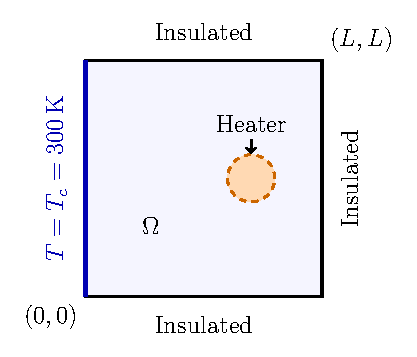
\includegraphics[width=\textwidth]{heat_theta_domain.pdf}
\end{column}
\begin{column}{0.58\textwidth}
On $\Omega=(0,L)^2$, $L=0.1\,\mathrm m$, solve
\[
\begin{cases}
\rho c\,\partial_tT-\nabla\cdot(k\nabla T)=r
&\text{in }\Omega,\\
T=T_c&\text{on the left edge},\\
k\nabla T\cdot\bm n=0&\text{on the other edges},\\
T(\bx,0)=T_c&\text{in }\Omega.
\end{cases}
\]
The heater remains on for $0<t\le60\,\mathrm s$.
The broad faces are insulated, and temperature is assumed uniform through the thickness.
\end{column}
\end{columns}
\end{frame}

\begin{frame}{Material properties and heater}
Use constant properties representative of an aluminum plate:
\[
k=200\,\mathrm{W/(m\,K)},\quad
\rho=2700\,\mathrm{kg/m^3},\quad c=900\,\mathrm{J/(kg\,K)}.
\]
The thermal diffusivity is
\[
\boxed{\alpha=\frac{k}{\rho c}=8.23\times10^{-5}\,\mathrm{m^2/s}.}
\]
Model the heater by a spatially concentrated heat supply:
\[
r(x,y)=r_0\exp\left[-\frac{(x-x_H)^2+(y-y_H)^2}{2w^2}\right],
\]
where $r_0=2\times10^6\,\mathrm{W/m^3}$,
$(x_H,y_H)=(0.07,0.05)\,\mathrm m$, and $w=0.01\,\mathrm m$.
For a $1\,\mathrm{mm}$ plate, this supplies approximately $1.3\,\mathrm W$.
\end{frame}

\begin{frame}{The time-step equation for this plate}
The insulated edges contribute zero boundary flux, and the heater is constant in time:
\[
\ell_T(v_h)=\int_\Omega r(\bx)v_h\,\dd x.
\]
The general $\theta$ equation therefore reduces to
\[
\begin{aligned}
m(T_h^{n+1},v_h)+\theta\Delta t\,a_T(T_h^{n+1},v_h)
={}&m(T_h^n,v_h)\\
&-(1-\theta)\Delta t\,a_T(T_h^n,v_h)
+\Delta t\,\ell_T(v_h).
\end{aligned}
\]
For backward Euler, $\theta=1$:
\[
\boxed{m(T_h^{n+1},v_h)+\Delta t\,a_T(T_h^{n+1},v_h)
=m(T_h^n,v_h)+\Delta t\,\ell_T(v_h).}
\]
At every step, impose $T_h^{n+1}=T_c$ on the left edge.
The unknown is the new temperature field.
\end{frame}

\begin{frame}{Implementation steps}
\textbf{Before the loop}
\begin{enumerate}
\item Create a triangular mesh and a continuous piecewise-linear FE space.
\item Prescribe $T_c$ on the left edge. Initialize $T_h^0=T_c$ everywhere.
\item Define the heater and the time-step forms.
\end{enumerate}
\medskip
\textbf{At every time step}
\begin{enumerate}
\item Solve the linear variational problem for $T_h^{n+1}$.
\item Copy its coefficients into the old temperature field.
\end{enumerate}
\medskip
The source and boundary values are fixed. Only the old temperature changes.
\end{frame}

\begin{frame}[fragile]{Notebook: material and boundary values}
\begin{lstlisting}
rho = 2700.0
c = 900.0
k = 200.0
alpha = k / (rho*c)
T_c = 300.0
\end{lstlisting}
The notebook creates a $24\times24$ rectangular grid divided into triangles
and uses degree-one Lagrange elements.
\begin{lstlisting}
boundary_dofs = fem.locate_dofs_geometrical(V, cooled_edge)
T_D = fem.Function(V)
T_D.x.array[:] = T_c
bc = fem.dirichletbc(T_D, boundary_dofs)
T_n = fem.Function(V)
T_n.x.array[:] = T_c
\end{lstlisting}
\texttt{cooled\_edge} selects $x=0$. The initial field and cooled edge both have temperature $T_c$.
\end{frame}

\begin{frame}[fragile]{Notebook: source and spatial forms}
With UFL coordinates \texttt{x[0]} and \texttt{x[1]}, define the same heater:
\begin{lstlisting}
r = r0*ufl.exp(-((x[0]-x_H)**2
                 + (x[1]-y_H)**2)/(2*w**2))

def m(S, v):
    return rho*c*S*v*dx

def a_T(S, v):
    return rho*c*alpha*ufl.inner(ufl.grad(S), ufl.grad(v))*dx
\end{lstlisting}
Here $\rho c\alpha=k$. The diffusivity enters the conduction term explicitly.
The notebook defines \texttt{S} and \texttt{v} as the UFL trial and test functions.
\end{frame}

\begin{frame}[fragile]{Notebook: time-step forms and solver}
The bilinear and linear forms directly match the time-step equation:
\begin{lstlisting}
A = m(S, v) + theta*dt*a_T(S, v)
L = m(T_n, v) - (1-theta)*dt*a_T(T_n, v) + dt*r*v*dx

problem = LinearProblem(
    A, L, bcs=[bc], petsc_options_prefix="heat_step_",
    petsc_options={"ksp_type": "preonly", "pc_type": "lu"})
\end{lstlisting}
\texttt{A} is the bilinear form for the new field.
\texttt{L} uses the known old field and heater.
\texttt{LinearProblem} assembles the system, enforces the cooled-edge
temperature, and solves it with direct LU factorization.
\end{frame}

\begin{frame}[fragile]{Notebook: the time loop}
For backward Euler, use $\theta=1$, $\Delta t=2\,\mathrm s$, and 30 steps:
\begin{lstlisting}
T_n.x.array[:] = T_c

for n in range(num_steps):
    T_new = problem.solve()
    T_n.x.array[:] = T_new.x.array
    time = (n+1)*float(dt.value)
\end{lstlisting}
Before the solve, \texttt{T\_n} holds $T_h^n$.
The solve gives $T_h^{n+1}$. The copy makes it the old field for the next step.
\medskip

The notebook also saves copies at 10, 30, and 60 seconds for plotting.
Those lines record results and do not change the algorithm.
\end{frame}

\begin{frame}{Computed temperatures}
\centering
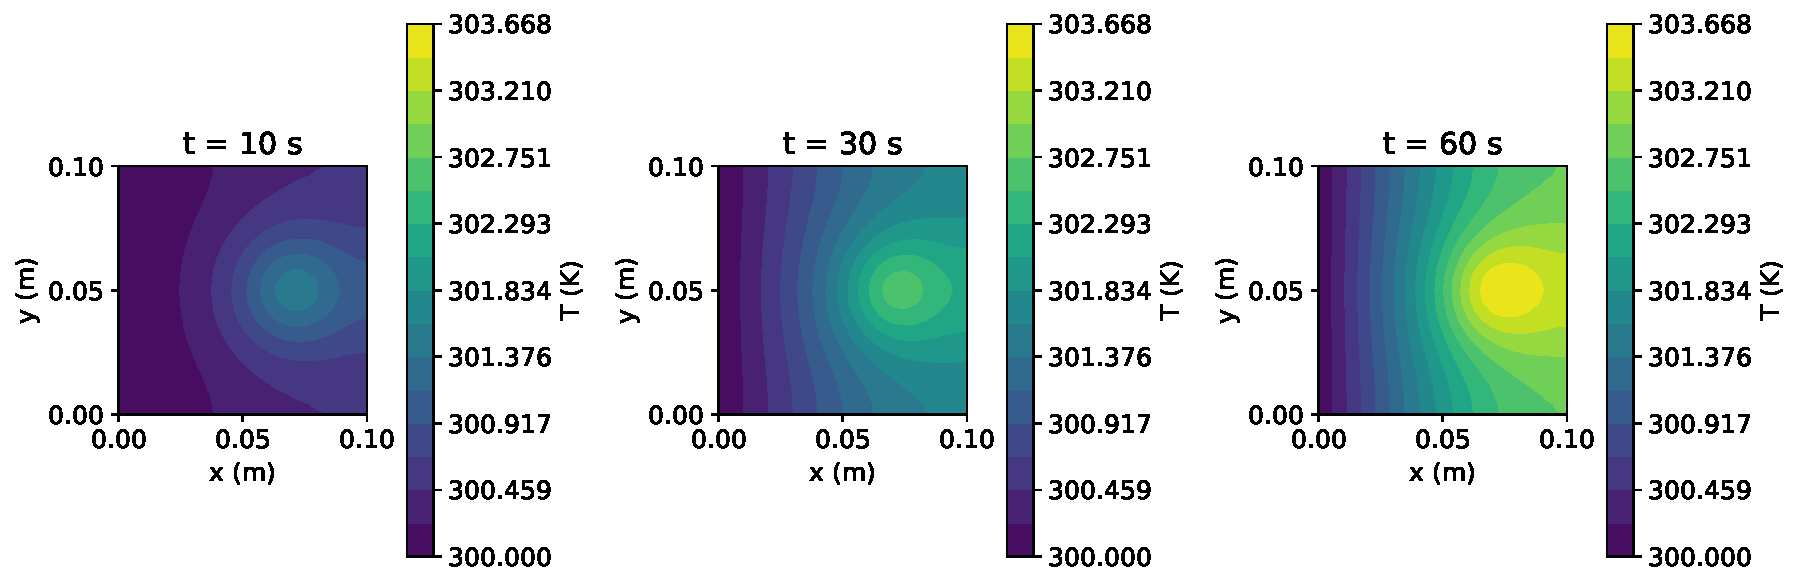
\includegraphics[width=0.99\textwidth]{heat_theta_solution.pdf}
\par\raggedright
All panels use the same temperature scale.
The heater raises the temperature locally, and conduction carries heat toward
the cooled left edge. With $\Delta t=2\,\mathrm s$, the maximum at 60 seconds is $303.668\,\mathrm K$.
\end{frame}

\begin{frame}{Time-step comparison}
In the notebook, repeat backward Euler with
\[
\Delta t=4,\ 2,\ 1\,\mathrm s
\]
on the same mesh, starting from $T_c$ every time.
Compare the maximum temperature and the change in the final field:
\begin{center}
\begin{tabular}{cc}
\toprule
$\Delta t$ (s) & Maximum $T$ at 60 s (K)\\
\midrule
$4$ & $303.639$\\
$2$ & $303.668$\\
$1$ & $303.683$\\
\bottomrule
\end{tabular}
\end{center}
\[
D=\left(\int_\Omega
[T_{h,\Delta t}(\bx,60)-T_{h,2\Delta t}(\bx,60)]^2\,\dd x\right)^{1/2}.
\]
This tests how much the computed temperature changes when the time step is halved.
A separate mesh-refinement study tests the spatial approximation.
\end{frame}

\begin{frame}{Summary}
\begin{itemize}
\item The material quantities remain explicit:
$\alpha=k/(\rho c)$ controls thermal diffusion.
\item The nonzero heater enters the load integral. The insulated edges
contribute zero normal-flux terms.
\item Each time step solves for the new temperature, then copies its coefficients into the old field.
\item Smaller time steps should be checked through changes in the computed solution.
\end{itemize}
\medskip
The complete implementation is in
\texttt{notebooks/transient/heat\_theta.ipynb}.
\end{frame}

\begin{frame}{References}
\begin{itemize}
\item Larson and Bengzon, \emph{The Finite Element Method: Theory,
Implementation, and Practice}, 2010 notes, Chapter 5,
\S\S5.1.4--5.1.5, pp.~99--101: spatial FE equations and time stepping.
\item Arnold, \emph{Lecture Notes on Numerical Analysis of Partial
Differential Equations}, Chapter 5, \S3, pp.~93--94: FE heat equations.
\item \href{https://jsdokken.com/dolfinx-tutorial/stable/chapter2/heat_code.html}
{Dokken, FEniCSx heat-equation tutorial}.
\item \href{https://docs.fenicsproject.org/dolfinx/v0.11.0/python/generated/dolfinx.fem.petsc.html}
{DOLFINx \texttt{LinearProblem} documentation}.
\end{itemize}
\end{frame}
\end{document}
